\begin{frame}
\frametitle{General supervised learning setting}
We have a training dataset of $n$ observations, each consisting of an input ${\bf x}_i$ and a target $y_i$.\par
Each input, ${\bf x}_i$, consists of a vector of $p$ features.
\begin{align*}
\mathcal{D} = \{({\bf x}_i,y_i) | i=1,..,n\}
\end{align*}

The aim is to predict the target for a new input ${\bf x}_*$.
\end{frame}

\begin{frame}
\frametitle{Classification}
\begin{columns}
\column{0.4\textwidth}
Targets (${\bf y}$) are categorical labels.\par
Train with $\mathcal{D}$ and use result to make best guess of $y_*$ given ${\bf x}_*$.
\column{0.6\textwidth}
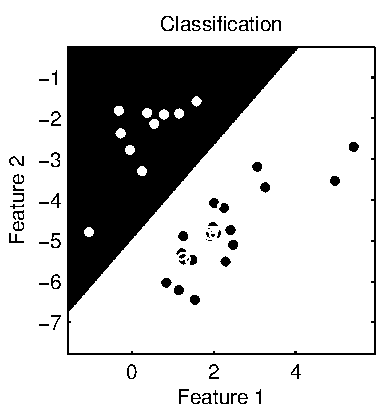
\includegraphics[width=\textwidth]{simple_classification}
\end{columns}
\end{frame}

\begin{frame}
\frametitle{Probabilistic classification}
\begin{columns}
\column{0.4\textwidth}
Targets (${\bf y}$) are categorical labels.\par
Train with $\mathcal{D}$ and compute $P(y_*=k | {\bf x}_*, \mathcal{D})$.
\column{0.6\textwidth}
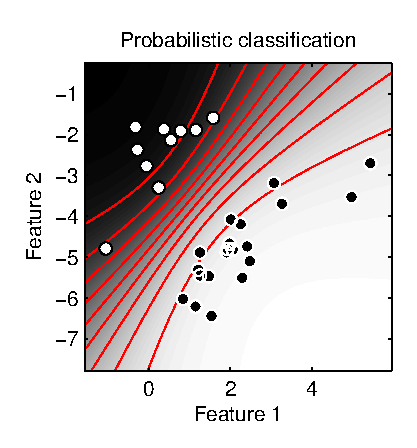
\includegraphics[width=\textwidth]{probabilistic_classification}
\end{columns}
\end{frame}

\begin{frame}
\frametitle{Regression}
\begin{columns}
\column{0.4\textwidth}
Targets (${\bf y}$) are continuous real variables.\par
Train with $\mathcal{D}$ and compute $p(y_* | {\bf x}_*, \mathcal{D})$.
\column{0.6\textwidth}
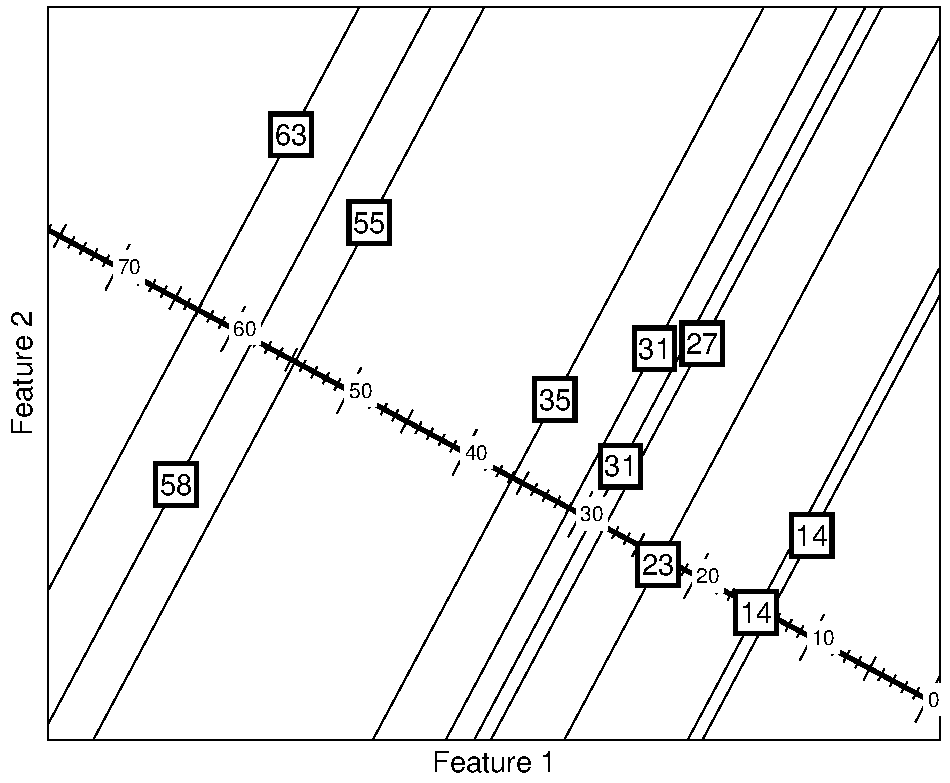
\includegraphics[width=\textwidth]{regression}
\end{columns}
\end{frame}

\begin{frame}
\frametitle{Many other settings}
\begin{itemize}
\item {\bf Multi-class classification} when there are more than two possible categories.
\item {\bf Ordinal regression} for classification when there is some ordering of the categories.\par
\begin{tiny}
Chu, Wei, and Zoubin Ghahramani. ``Gaussian processes for ordinal regression.'' In Journal of Machine Learning Research, pp. 1019-1041. 2005.\par
\end{tiny}
\item {\bf Multi-task learning} when there are multiple targets to predict, which may be related.
\item etc
\end{itemize}
\end{frame}

\begin{frame}
\frametitle{Multi-Class classification}

\begin{columns}
\column{.5\textwidth}
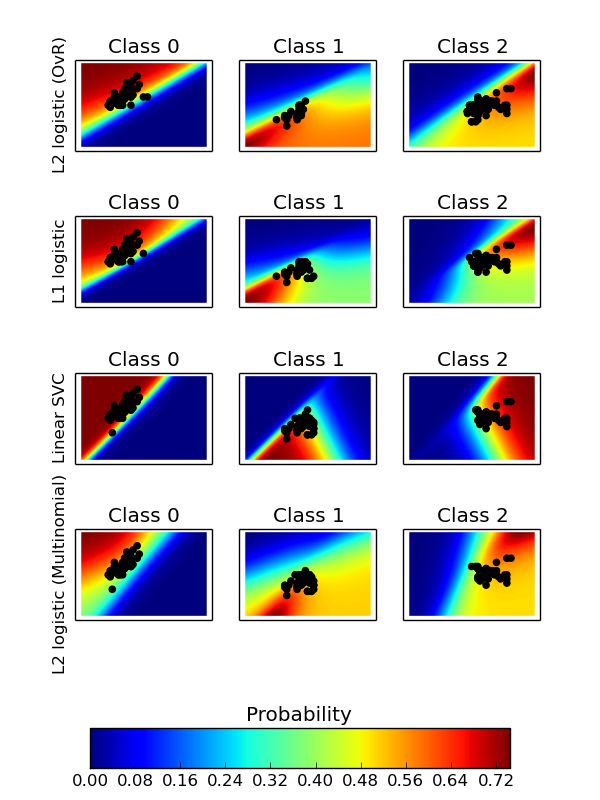
\includegraphics[width=\textwidth]{sklearn_material/plot_classification_probability_001.png}
\column{.6\textwidth}
\begin{itemize}
\item {\bf Multinomial Logistic regression} Theoretically optimal. Expensive optimization. 
\item {\bf One-versus-all classification} [SVMs] Among several
  hyperplane, choose the one with maximal margin. \\$\Longrightarrow$
  recommended
\item {\bf One-versus-one classification} Vote across each pair of
  class. Expensive, not optimal.
\end{itemize}
\end{columns}
\end{frame}

